\section{Критическое поведение модели IsingISAW на треугольной решётке}

В данном разделе проводится исследование критической области модели Изинга на случайном блуждания без самопересечений на треугольной решётке (далее, TrIsingISAW).
В отличие от классической модели на квадратной решётке, узлы треугольной решётки имеют две дополнительные связи по одной из диагоналей (см. рисунок \ref{fig:lattices}), 
вследствие чего координационное число данной модификации (кол-во возможных связей у одного узла) увеличено по сравнению с квадратной с 4 до 6.

\subsection{Поиск точки фазового перехода}

\begin{equation}
\label{eq:IsISAW_H}
 H_{N,u,\{\sigma\}} = -\sum_{i,j} J\sigma_i \sigma_j, i,j \in u, |u| = N
\end{equation}

\begin{equation}
\label{eq:TrIsISAW_E}
\la \epsilon \ra = \la H \ra / N
\end{equation}

Были проведены симуляции Монте-Карло при нулевом внешнем поле и $J \in [0,0.9]$. 
Итоговое количество шагов симуляций от $10^10$ до $10^11$, симулированные блуждания имеют длину $N$ от 100 до 7200.
Были собраны данные для удельной энергии системы на спин $\la \epsilon \ra$ \eqref{eq:TrIsISAW_E} и средняя 2-я и 4-я степени намагниченности на спин $\la m^2 \ra$, $\la m^4 \ra$.
Так же собрана статистика среднего расстояния между концами блуждания $R^2_N$.

\begin{figure}[h]
\begin{subfigure}{0.49\textwidth}
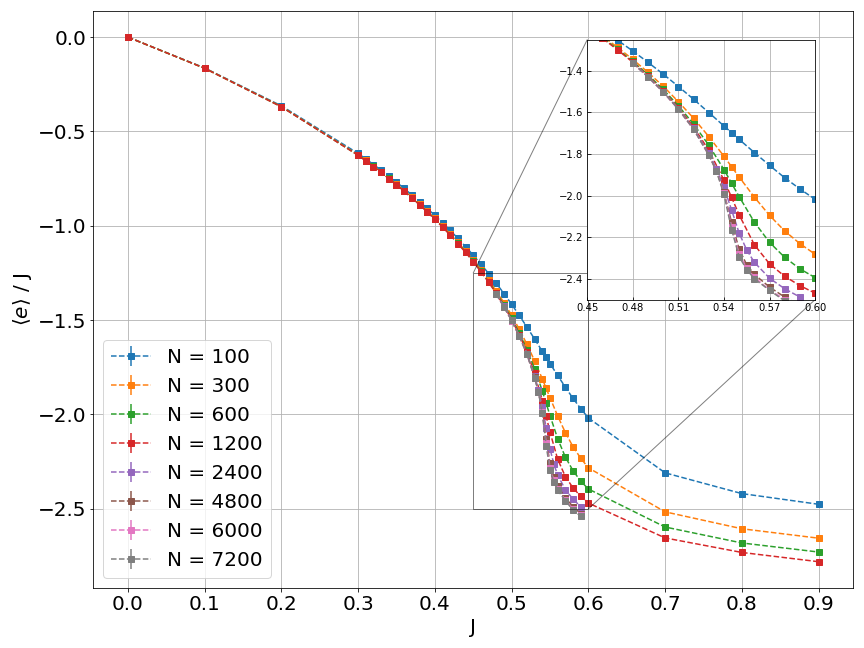
\includegraphics[width=\textwidth]{TrIsISAW_E.png}
\end{subfigure}
\hfill
\begin{subfigure}{0.49\textwidth}
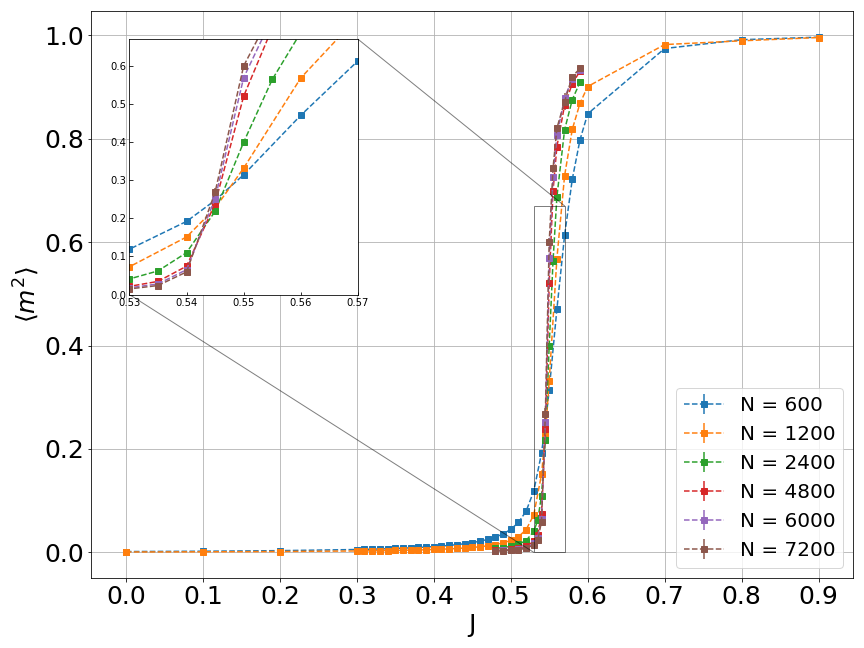
\includegraphics[width=\textwidth]{TrIsISAW_m2.png}
\end{subfigure}
\caption{Слева: удельная энергия узла \eqref{eq:TrIsISAW_E} модели TrIsingISAW (без учёта константы $J$). Справа: средняя вторая степень намагниченности узла модели TrIsingISAW. Длины конформаций в обоих графиках от 100 до 7200 (длины отмечены разными цветами)}
\label{fig:TrIsISAW_E}
\end{figure}

На графике \ref{fig:TrIsISAW_E} показана зависимость удельной энергии \eqref{eq:TrIsISAW_E} узла модели TrIsingISAW.
График показывает что удельная энергия системы стремится к -3J в пределе бесконечной длины конформации, 
что логично, поскольку с ростом $J$ узлы приобретают наиболее возможное число связей (то есть, 6), но так как св
язи существуют между парами узлов,
необходимо поделить число связей на 2.
При малых $J$ энергия почти не зависит от длины цепочки $N$, но начиная с $J > 0.53$, расхождение графиков становится наиболее четким.

\begin{equation}
\label{eq:IsISAW_m2}
	m^{k} = (\sum_{i \in u} \sigma_i / N)^k
\end{equation}

На графике \ref{fig:TrIsISAW_m2} изображен момент намагниченности второго порядка \eqref{eq:IsISAW_m2} в зависимости от $J$.
Графики величины для конформаций разных длин имеют четкое пересечение в $J \approx 0.545$.

\begin{equation}
\label{eq:IsISAW_U4}
	U_4 = 1 - \frac{\la m^4 \ra}{3 \la m^2 \ra}
\end{equation}

\begin{figure}[h]
\begin{subfigure}{0.49\textwidth}
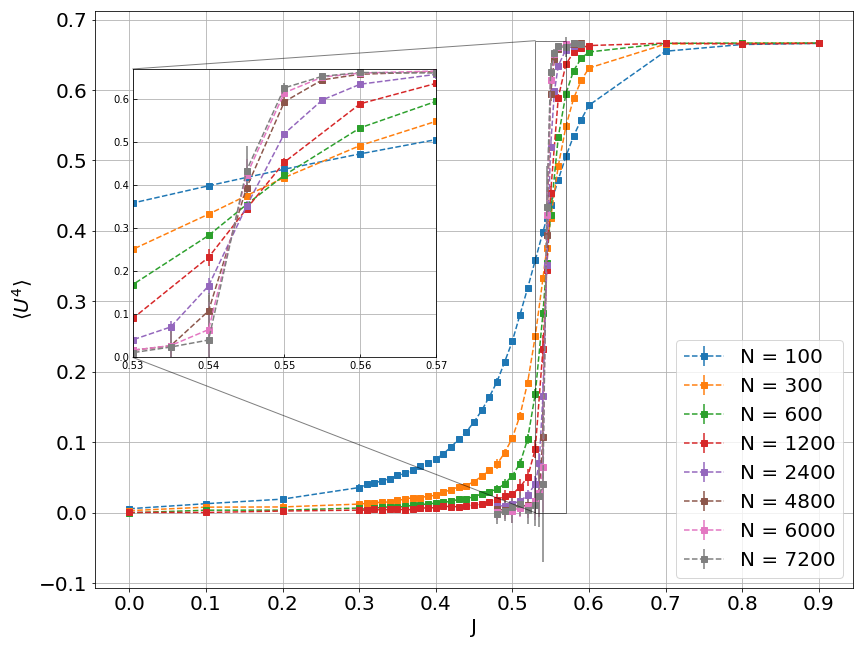
\includegraphics[width=\textwidth]{TrIsISAW_U4.png}
\end{subfigure}
\hfill
\begin{subfigure}{0.49\textwidth}
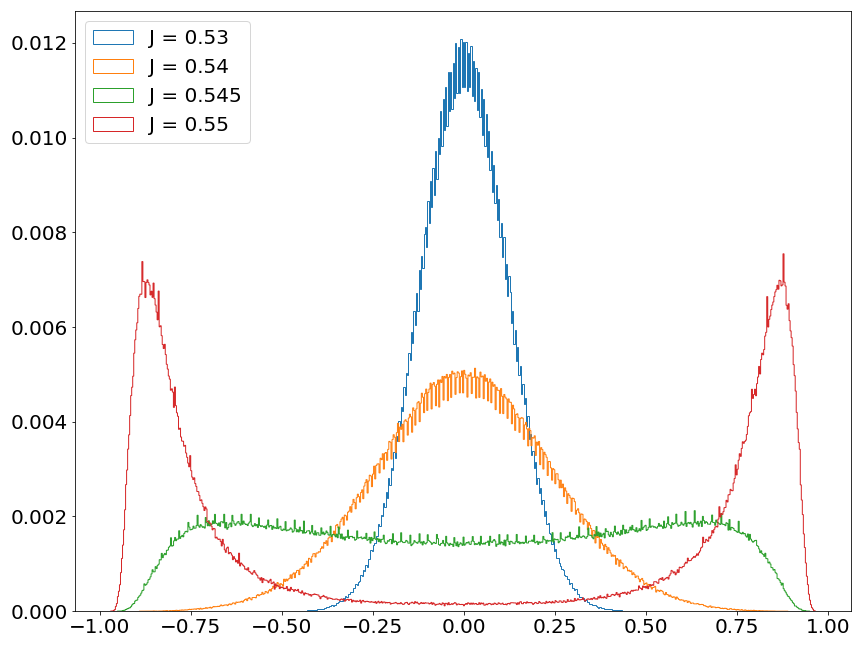
\includegraphics[width=\textwidth]{TrIsISAW_m2_distr.png}
\end{subfigure}
\caption{Слева: кумулянт Биндера модели TrIsingISAW с длиной конформации от 100 до 7200 (длины отмечены разными цветами).
Справа: распределение удельной намагниченности модели TrIsingISAW на конформации длиной $N=7200$ при $J \in [0.53,0.55]$ (значения J отмечены разными цветами)}
\label{fig:TrIsISAW_E}
\end{figure}


График \ref{fig:TrIsISAW_U4} показывает зависость кумулянта Биндера \eqref{eq:IsISAW_U4} от J. 
Пересечение графиков от конформаций разных длин, соответствующее переходу от парамагнетических к ферромагнетическим свойствам, снова наблюдается в $J \approx 0.545$.

Распределение значений удельной намагниченности для модели TrIsingISAW изображено на графике \ref{fig:TrIsISAW_m2_distr}.
График показывает, что распределение с преобладающими малыми по модулю значениями удельной намагниченности уступают 
распределениям с преобладающими крайними значениями намагниченности возле $J=0.545$, где распределение близко к почти равномерному.

На основании рассмотренных величин и протекаемых по ним переходов, оценка точки фазового перехода следующая:

\begin{equation}
	J_c = 0.545(5)
\end{equation}

Для оценки критического кумулянта, ввиду слишком большой наблюдаемой погрешности, требуются более длительные симуляции длин $N > 5000$.

\newpage

\subsection{Необсуждённые графики}

\begin{figure}[h]
\centering
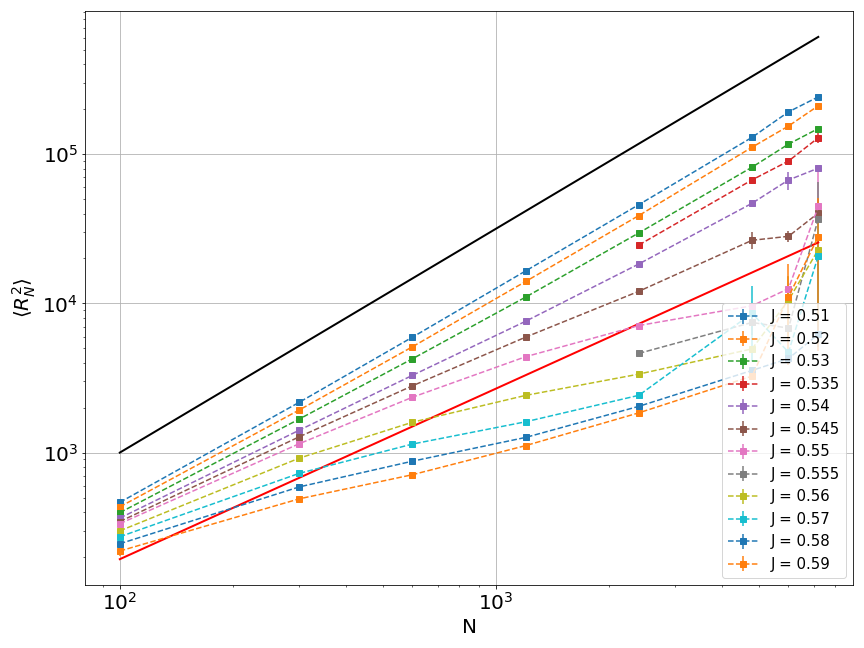
\includegraphics[width=0.7\textwidth]{TrIsISAW_R2log.png}
\caption{Расстояние между концами блужданий конформаций от длины $N$ при $J \in [0.51,0.59]$ в логарифмическом масштабе. 
Для наглядности добавлены линии $N^{2v}$, где $v = 4/7$ (красная линия) и $v=3/4$ (чёрная линия).}
\label{fig:TrIsISAW_R2log}
\end{figure}

